\section{Algorithms}\label{sec:algorithms}

In this section, we will describe a set of algorithms that can be easily incorporated into
standard numerical solvers, and that ensure that the resulting discrete de Rham complex
remains exact after local refinement.

The main algorithm is \Cref{alg:exact-mesh}, which takes as input a hierarchical space, 
described by its basis \(\thbbasis^{\boldvec{0}}_{L}\), and a set of elements marked for
refinement, and returns an updated basis that leads to an exact complex.
The algorithm is subdivided into five steps, the first three  corresponding to
\Cref{alg:initiate-unchecked,alg:nlintersec,alg:shortest-chain}.

The first step is to obtain the basis functions that need to be checked for problematic
pairs.
Here, we compute the basis functions in \(\Bll\) and then use \Cref{lem:problematic-sides}
to discard basis functions that are resolved in some direction, to remove unnecessary
computations.
Then, we loop over all unordered pairs of relevant basis functions 
and use
\Cref{alg:nlintersec,alg:shortest-chain} to check if the pair is problematic, comprising
steps two and three.
See \Cref{fig:problematic-pair-algorithm-illustration} for an
illustration.

\Cref{alg:nlintersec} performs the check for a \nlintersec between the pair using
\Cref{def:nlintersec}.
It first calls the method \var{get\_support\_per\_dim}, that computes the
breakpoint-interval indices of the intervals where a basis function is supported, in each
dimension, as defined in \eqref{eq:breakpoint-indices}; concretely, if the support of
\(\bsp\) in dimension \(k\) contains only the intervals
\((\zeta_i,\zeta_{i+1}),\dots,(\zeta_j,\zeta_{j+1})\), for some \(i,j\), then
\var{get\_support\_per\_dim} would return the integers \(\{i,\dots,j+1\}\).
Then, the algorithm computes the intersection of the supports of the pair of basis
functions, and by working with the integer indices of the intervals the subsequent
computations are cheaper than if using real values.
Another method used in this algorithm that should be implemented is
\var{get\_contained\_indices}, which returns the biggest subset of \(\knotvec_{(\level+1,
k)}\) contained in the intersection of the pair's supports, for a given dimension \(k\) and
level \(\level\).

The \Cref{alg:shortest-chain} used in the third step assumes that the given pair of basis
functions shares a \nlintersec, since this is the appropriate case for
\Cref{alg:exact-mesh}, and it makes the check of a direction-\(k\) chain between the pair
trivial.
If no such chain exists, we then construct the interaction box, as in
\Cref{def:int-box}, and check if there is a shortest chain between the pair using
\Cref{lem:int-box-chain}.
To do this, we chose to implement the interaction box as a graph ―
in this case, a subgraph of a lattice graph ― and then use a standard algorithm to check if
a path exists between nodes on a graph, named as \var{has\_chain} in the algorithm.
Packages that perform these operations are commonplace and should be available in most
programming languages.

We reach the fourth step when a pair of B-splines is problematic. 
In this case, we use the method \var{get\_lchain\_indices} to select what L-chain should be
added, according to \Cref{rem:preferable-lchain}, and return all the indices of the basis
functions in the \lchain and its corner function.
This information is used to update the basis functions and marked elements used in the next
iteration of checking for problematic pairs.

The last step consists of computing all the new pairs that will need to be checked,
taking into account those that were already fixed with the added \lchains, and updating the
hierarchical basis accordingly.

Finally, steps two to five are repeated until there are no more problematic pairs in the
hierarchical basis.

\begin{rem}
	\Cref{alg:exact-mesh} can be adapted to enforce an admissible
	\(\hbspace^{\boldvec{0}}_{L}\) with few alterations.
	Notice that the addition of \lchains only affects the elements marked for refinement at
	a given level \(\level\), and the imposition of admissibility the elements at levels
	below \(\level\). 
	Therefore, we can reverse the outermost loop in the algorithm, starting from the finer
	level and going down to the coarsest level, and perform the admissibility imposition
	after all the problematic pairs at a given level have been fixed.
	This way, we ensure that any possible problematic pair introduce by the addition of
	admissibility will still be fixed in the following iterations.
\end{rem}

\begin{algorithm}[H]
    \caption{Exact mesh refinement.}
    \label{alg:exact-mesh}
	\begin{algorithmic}[1]
		\Require \(\thbbasis^{\boldvec{0}}_{L}\), a set of marked elements to refine per
		level \var{marked\_els}
		\Ensure Updated truncated hierarchical basis \(\thbbasis^{\boldvec{0}}_{L}\) with no
		problematic intersections
		\ForAll{\(\level \var{ in } \{0,\dots,L-1\}\)}
			\State \(\var{unchecked\_pairs} \gets
				\var{initiate\_unchecked\_pairs}(\thbbasis^{\boldvec{0}}_{L},
				\level, \var{marked\_els})\)
			\State \(\var{checked\_pairs} \gets \emptyset\)
			\State \(\var{problematic\_mesh} \gets \var{true}\)
			\Statex
			\While{\var{problematic\_mesh}}
				\State  \(\var{problematic\_mesh} \gets \var{false}\)
				\Statex
				\ForAll{\var{pair in unchecked\_pairs}}
					\State \(\var{has\_min\_intersec} \gets
					\var{has\_minimal\_intersection}(\thbbasis^{\boldvec{0}}_{L}, \level,
					\var{pair})\)
					\If{\(\neg \var{has\_min\_intersec}\)}
						\State \var{skip iteration}
					\EndIf
					\Statex
					\State \(\var{has\_no\_chain} \gets
						\neg\var{has\_shortest\_chain}(\thbbasis^{\boldvec{0}}_{L}, \level,
						\var{pair})\)
					\If{\var{has\_no\_chain}}
						\State \var{lchain, corner\_func} \(\gets\)
							\var{get\_lchain\_indices}(\(\thbbasis^{\boldvec{0}}_{L}\),
							\(\level\), pair)
						\State \var{unchecked\_funcs} \(\gets\) \var{unchecked\_funcs} \(\cup\)
							\var{corner\_func}
						\State \var{marked\_els[\(\level\)]} \(\gets\)
							\var{marked\_els[\(\level\)]} \(\cup\)
							\var{get\_support(lchain)}
						\State  \(\var{problematic\_mesh} \gets \var{true}\)
					\EndIf
				\EndFor
				\Statex
				\State \var{checked\_pairs} \(\gets\) \var{checked\_pairs} \(\cup\)
					\var{unchecked\_pairs}
				\State \var{unchecked\_pairs} \(\gets\)
					\var{combinations}(\var{unchecked\_funcs},
					2) 
				\State \(\var{unchecked\_pairs} \gets \var{unchecked\_pairs} \backslash
				\var{checked\_pairs}\)
				\State \(\thbbasis^{\boldvec{0}}_{L} \gets\)
					\var{update\_hierarchical\_space}(\(\thbbasis^{\boldvec{0}}_{L}\),
					\var{marked\_els})
			\EndWhile
		\EndFor

		\State \Return \(\thbbasis^{\boldvec{0}}_{L}\)
	\end{algorithmic}
\end{algorithm}

\begin{algorithm}[H]
    \caption{\var{initiate\_unchecked\_pairs}}
    \label{alg:initiate-unchecked}
	\begin{algorithmic}[1]
		\Require 	
        \(\thbbasis^{\boldvec{0}}_{L}\),
        hierarchical level \(\level\),
        set of marked elements to refine per level \var{marked\_els}
		\Ensure pairs of basis functions that might be problematic 
		\State \(\domain_{\level+1} \gets \domain_{\level+1} \cup \var{marked\_els}\)
		\State \(\var{supported\_funcs} \gets \Bll\)
		\Comment{As defined in \Cref{sec:exact-meshes}.}
		\State \var{unchecked\_funcs} \(\gets \emptyset\)
		\ForAll{\(\xbsp_{\boldvec{i}} \in \var{supported\_funcs}\)}
			\ForAll{\(k \var{ in } \{1,2\}\)}
				\If{\(\xbsp_{\boldvec{i}}\) is resolved in \(k\)}
					\State \var{skip iteration}
					\Comment{Using \Cref{lem:problematic-sides}.}
				\EndIf
			\EndFor
			\State \var{unchecked\_funcs} \(\gets \var{unchecked\_funcs} \cup
			\xbsp_{\boldvec{i}}\)
		\EndFor
		\State \(\var{unchecked\_pairs} \gets
			\var{combinations}(\var{unchecked\_funcs},2)\)
			\ForAll{\((\xbsp_{\boldvec{i}}, \xbsp_{\boldvec{j}})\) \var{in} \var{unchecked\_pairs}}
			\If{\(\supp(\xbsp_{\boldvec{i}})\cap \var{marked\_els} == \emptyset\)
			\var{ and }\(\supp(\xbsp_{\boldvec{j}})\cap \var{marked\_els} == \emptyset\)}
				\State \var{unchecked\_pairs} \(\gets\) \var{unchecked\_pairs}
				\(\backslash\) \((\xbsp_{\boldvec{i}}, \xbsp_{\boldvec{j}})\)
			\EndIf
		\EndFor

		\State \Return \var{unchecked\_pairs}
	\end{algorithmic}
\end{algorithm}

\begin{algorithm}[H]
	\caption{\var{has\_minimal\_intersection} (Checks if there is a \nlintersec between a pair of
	B-splines.)}
    \label{alg:nlintersec}
	\begin{algorithmic}[1]
		\Require \(\thbbasis^{\boldvec{0}}_{L}\), \var{pair} = \(
		(\xbsp_{\boldvec{i}}, \xbsp_{\boldvec{j}})
		\), hierarchical level \(\level\).
		\Ensure Boolean indicating if the pair shares a \nlintersec.
		\State \var{supp\_bi} \(\gets\) \var{get\_support\_per\_dim}
		(\(\xbsp_{\boldvec{i}}\))
		\State \var{supp\_bj} \(\gets\) \var{get\_support\_per\_dim}
		(\(\xbsp_{\boldvec{j}}\))
		\ForAll{\(k \var{ in } \{1, 2\}\)}
			\State \var{supp\_intersection} \(\gets\) \var{supp\_bi[k]} \(\cap\)
			\var{supp\_bj[k]}
			\If{\var{supp\_intersection}\;==\;\(\emptyset\)}
				\State \Return \var{false}
			\EndIf
			\State \(I_k \gets\) \var{get\_contained\_indices}(\var{supp\_intersection}, \(\knotvec_{(\level+1,k)}\))
			\Comment{At level \(\ell+1\).}
			\State \var{length\_flag[k]} \(\gets\)
				\var{length(\(I_k\))\;>\;\(p_{(\level+1,k)}\)}
			\Comment{Condition of \Cref{def:nlintersec}.}
		\EndFor
		\State \(\var{has\_min\_intersec} \gets \var{any}(\var{length\_flag})==\var{true}\)

		\State \Return \var{has\_min\_intersec}
	\end{algorithmic}
\end{algorithm}

\begin{algorithm}[H]
	\caption{
		\var{has\_shortest\_chain} (Checks if a pair of B-splines that share a
		\nlintersec have a shortest chain between them.)
	}
    \label{alg:shortest-chain}
	\begin{algorithmic}[1]
		\Require 
        \(\thbbasis^{\boldvec{0}}_{L}\),
		\var{pair} = \(
		(\xbsp_{\boldvec{i}}, \xbsp_{\boldvec{j}})
		\),
        hierarchical level \(\level\).
		\Ensure Boolean indicating if there is a shortest chain between the pair of
		B-splines.
		\If{\var{any}(\(\boldvec{i}-\boldvec{j}\))==0}
			\State \Return \var{true}
			\Comment{There is a direction-\(k\) chain.}
		\EndIf
		\State \var{inter\_box} \(\gets \interbox{\boldvec{i}}{\boldvec{j}}\)
		\Comment{As in \Cref{def:int-box}.}
		\If{\var{has\_chain(inter\_box, \(\boldvec{i}\), \(\boldvec{j}\))}}
			\State \Return \var{true}
			\Comment{Using \Cref{lem:int-box-chain}.}
		\Else
			\State \Return \var{false}
		\EndIf	
	\end{algorithmic}
\end{algorithm}

\begin{figure}[H]
    \centering
    \hfill
    \begin{subfigure}[t]{0.325\textwidth}
        \centering
        \input{problematic-pair-algorithm-case-1-illustration.tex}
        \caption{}
        \label{fig:problematic-pair-algorithm-case-1-illustration}
    \end{subfigure}
	\hfill
    \begin{subfigure}[t]{0.325\textwidth}
		\centering
		\input{problematic-pair-algorithm-case-2-illustration.tex}
		\caption{}
		\label{fig:problematic-pair-algorithm-case-2-illustration}
    \end{subfigure}
	\hfill
    \begin{subfigure}[t]{0.325\textwidth}
        \centering
        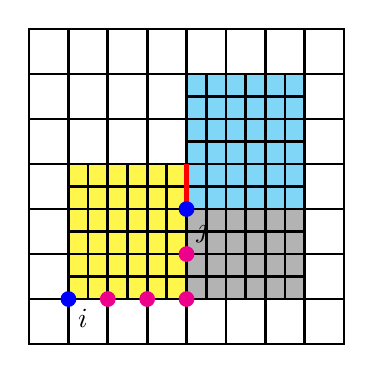
\begin{tikzpicture}[scale=4.0]
    % Define layers
    \pgfdeclarelayer{background}
    \pgfsetlayers{background,main}

    \coordinate (v1_1) at (0.0, 0.0);
    \coordinate (v1_2) at (0.125, 0.0);
    \coordinate (v1_3) at (0.125, 0.14285714285714285);
    \coordinate (v1_4) at (0.0, 0.14285714285714285);
    \draw[black, line width=1.0pt] (v1_1) -- (v1_2) -- (v1_3) -- (v1_4) -- cycle;
    \coordinate (v2_1) at (0.125, 0.0);
    \coordinate (v2_2) at (0.25, 0.0);
    \coordinate (v2_3) at (0.25, 0.14285714285714285);
    \coordinate (v2_4) at (0.125, 0.14285714285714285);
    \draw[black, line width=1.0pt] (v2_1) -- (v2_2) -- (v2_3) -- (v2_4) -- cycle;
    \coordinate (v3_1) at (0.25, 0.0);
    \coordinate (v3_2) at (0.375, 0.0);
    \coordinate (v3_3) at (0.375, 0.14285714285714285);
    \coordinate (v3_4) at (0.25, 0.14285714285714285);
    \draw[black, line width=1.0pt] (v3_1) -- (v3_2) -- (v3_3) -- (v3_4) -- cycle;
    \coordinate (v4_1) at (0.375, 0.0);
    \coordinate (v4_2) at (0.5, 0.0);
    \coordinate (v4_3) at (0.5, 0.14285714285714285);
    \coordinate (v4_4) at (0.375, 0.14285714285714285);
    \draw[black, line width=1.0pt] (v4_1) -- (v4_2) -- (v4_3) -- (v4_4) -- cycle;
    \coordinate (v5_1) at (0.5, 0.0);
    \coordinate (v5_2) at (0.625, 0.0);
    \coordinate (v5_3) at (0.625, 0.14285714285714285);
    \coordinate (v5_4) at (0.5, 0.14285714285714285);
    \draw[black, line width=1.0pt] (v5_1) -- (v5_2) -- (v5_3) -- (v5_4) -- cycle;
    \coordinate (v6_1) at (0.625, 0.0);
    \coordinate (v6_2) at (0.75, 0.0);
    \coordinate (v6_3) at (0.75, 0.14285714285714285);
    \coordinate (v6_4) at (0.625, 0.14285714285714285);
    \draw[black, line width=1.0pt] (v6_1) -- (v6_2) -- (v6_3) -- (v6_4) -- cycle;
    \coordinate (v7_1) at (0.75, 0.0);
    \coordinate (v7_2) at (0.875, 0.0);
    \coordinate (v7_3) at (0.875, 0.14285714285714285);
    \coordinate (v7_4) at (0.75, 0.14285714285714285);
    \draw[black, line width=1.0pt] (v7_1) -- (v7_2) -- (v7_3) -- (v7_4) -- cycle;
    \coordinate (v8_1) at (0.875, 0.0);
    \coordinate (v8_2) at (1.0, 0.0);
    \coordinate (v8_3) at (1.0, 0.14285714285714285);
    \coordinate (v8_4) at (0.875, 0.14285714285714285);
    \draw[black, line width=1.0pt] (v8_1) -- (v8_2) -- (v8_3) -- (v8_4) -- cycle;
    \coordinate (v9_1) at (0.0, 0.14285714285714285);
    \coordinate (v9_2) at (0.125, 0.14285714285714285);
    \coordinate (v9_3) at (0.125, 0.2857142857142857);
    \coordinate (v9_4) at (0.0, 0.2857142857142857);
    \draw[black, line width=1.0pt] (v9_1) -- (v9_2) -- (v9_3) -- (v9_4) -- cycle;
    \coordinate (v10_1) at (0.875, 0.14285714285714285);
    \coordinate (v10_2) at (1.0, 0.14285714285714285);
    \coordinate (v10_3) at (1.0, 0.2857142857142857);
    \coordinate (v10_4) at (0.875, 0.2857142857142857);
    \draw[black, line width=1.0pt] (v10_1) -- (v10_2) -- (v10_3) -- (v10_4) -- cycle;
    \coordinate (v11_1) at (0.0, 0.2857142857142857);
    \coordinate (v11_2) at (0.125, 0.2857142857142857);
    \coordinate (v11_3) at (0.125, 0.42857142857142855);
    \coordinate (v11_4) at (0.0, 0.42857142857142855);
    \draw[black, line width=1.0pt] (v11_1) -- (v11_2) -- (v11_3) -- (v11_4) -- cycle;
    \coordinate (v12_1) at (0.875, 0.2857142857142857);
    \coordinate (v12_2) at (1.0, 0.2857142857142857);
    \coordinate (v12_3) at (1.0, 0.42857142857142855);
    \coordinate (v12_4) at (0.875, 0.42857142857142855);
    \draw[black, line width=1.0pt] (v12_1) -- (v12_2) -- (v12_3) -- (v12_4) -- cycle;
    \coordinate (v13_1) at (0.0, 0.42857142857142855);
    \coordinate (v13_2) at (0.125, 0.42857142857142855);
    \coordinate (v13_3) at (0.125, 0.5714285714285714);
    \coordinate (v13_4) at (0.0, 0.5714285714285714);
    \draw[black, line width=1.0pt] (v13_1) -- (v13_2) -- (v13_3) -- (v13_4) -- cycle;
    \coordinate (v14_1) at (0.875, 0.42857142857142855);
    \coordinate (v14_2) at (1.0, 0.42857142857142855);
    \coordinate (v14_3) at (1.0, 0.5714285714285714);
    \coordinate (v14_4) at (0.875, 0.5714285714285714);
    \draw[black, line width=1.0pt] (v14_1) -- (v14_2) -- (v14_3) -- (v14_4) -- cycle;
    \coordinate (v15_1) at (0.0, 0.5714285714285714);
    \coordinate (v15_2) at (0.125, 0.5714285714285714);
    \coordinate (v15_3) at (0.125, 0.7142857142857143);
    \coordinate (v15_4) at (0.0, 0.7142857142857143);
    \draw[black, line width=1.0pt] (v15_1) -- (v15_2) -- (v15_3) -- (v15_4) -- cycle;
    \coordinate (v16_1) at (0.125, 0.5714285714285714);
    \coordinate (v16_2) at (0.25, 0.5714285714285714);
    \coordinate (v16_3) at (0.25, 0.7142857142857143);
    \coordinate (v16_4) at (0.125, 0.7142857142857143);
    \draw[black, line width=1.0pt] (v16_1) -- (v16_2) -- (v16_3) -- (v16_4) -- cycle;
    \coordinate (v17_1) at (0.25, 0.5714285714285714);
    \coordinate (v17_2) at (0.375, 0.5714285714285714);
    \coordinate (v17_3) at (0.375, 0.7142857142857143);
    \coordinate (v17_4) at (0.25, 0.7142857142857143);
    \draw[black, line width=1.0pt] (v17_1) -- (v17_2) -- (v17_3) -- (v17_4) -- cycle;
    \coordinate (v18_1) at (0.375, 0.5714285714285714);
    \coordinate (v18_2) at (0.5, 0.5714285714285714);
    \coordinate (v18_3) at (0.5, 0.7142857142857143);
    \coordinate (v18_4) at (0.375, 0.7142857142857143);
    \draw[black, line width=1.0pt] (v18_1) -- (v18_2) -- (v18_3) -- (v18_4) -- cycle;
    \coordinate (v19_1) at (0.875, 0.5714285714285714);
    \coordinate (v19_2) at (1.0, 0.5714285714285714);
    \coordinate (v19_3) at (1.0, 0.7142857142857143);
    \coordinate (v19_4) at (0.875, 0.7142857142857143);
    \draw[black, line width=1.0pt] (v19_1) -- (v19_2) -- (v19_3) -- (v19_4) -- cycle;
    \coordinate (v20_1) at (0.0, 0.7142857142857143);
    \coordinate (v20_2) at (0.125, 0.7142857142857143);
    \coordinate (v20_3) at (0.125, 0.8571428571428571);
    \coordinate (v20_4) at (0.0, 0.8571428571428571);
    \draw[black, line width=1.0pt] (v20_1) -- (v20_2) -- (v20_3) -- (v20_4) -- cycle;
    \coordinate (v21_1) at (0.125, 0.7142857142857143);
    \coordinate (v21_2) at (0.25, 0.7142857142857143);
    \coordinate (v21_3) at (0.25, 0.8571428571428571);
    \coordinate (v21_4) at (0.125, 0.8571428571428571);
    \draw[black, line width=1.0pt] (v21_1) -- (v21_2) -- (v21_3) -- (v21_4) -- cycle;
    \coordinate (v22_1) at (0.25, 0.7142857142857143);
    \coordinate (v22_2) at (0.375, 0.7142857142857143);
    \coordinate (v22_3) at (0.375, 0.8571428571428571);
    \coordinate (v22_4) at (0.25, 0.8571428571428571);
    \draw[black, line width=1.0pt] (v22_1) -- (v22_2) -- (v22_3) -- (v22_4) -- cycle;
    \coordinate (v23_1) at (0.375, 0.7142857142857143);
    \coordinate (v23_2) at (0.5, 0.7142857142857143);
    \coordinate (v23_3) at (0.5, 0.8571428571428571);
    \coordinate (v23_4) at (0.375, 0.8571428571428571);
    \draw[black, line width=1.0pt] (v23_1) -- (v23_2) -- (v23_3) -- (v23_4) -- cycle;
    \coordinate (v24_1) at (0.875, 0.7142857142857143);
    \coordinate (v24_2) at (1.0, 0.7142857142857143);
    \coordinate (v24_3) at (1.0, 0.8571428571428571);
    \coordinate (v24_4) at (0.875, 0.8571428571428571);
    \draw[black, line width=1.0pt] (v24_1) -- (v24_2) -- (v24_3) -- (v24_4) -- cycle;
    \coordinate (v25_1) at (0.0, 0.8571428571428571);
    \coordinate (v25_2) at (0.125, 0.8571428571428571);
    \coordinate (v25_3) at (0.125, 1.0);
    \coordinate (v25_4) at (0.0, 1.0);
    \draw[black, line width=1.0pt] (v25_1) -- (v25_2) -- (v25_3) -- (v25_4) -- cycle;
    \coordinate (v26_1) at (0.125, 0.8571428571428571);
    \coordinate (v26_2) at (0.25, 0.8571428571428571);
    \coordinate (v26_3) at (0.25, 1.0);
    \coordinate (v26_4) at (0.125, 1.0);
    \draw[black, line width=1.0pt] (v26_1) -- (v26_2) -- (v26_3) -- (v26_4) -- cycle;
    \coordinate (v27_1) at (0.25, 0.8571428571428571);
    \coordinate (v27_2) at (0.375, 0.8571428571428571);
    \coordinate (v27_3) at (0.375, 1.0);
    \coordinate (v27_4) at (0.25, 1.0);
    \draw[black, line width=1.0pt] (v27_1) -- (v27_2) -- (v27_3) -- (v27_4) -- cycle;
    \coordinate (v28_1) at (0.375, 0.8571428571428571);
    \coordinate (v28_2) at (0.5, 0.8571428571428571);
    \coordinate (v28_3) at (0.5, 1.0);
    \coordinate (v28_4) at (0.375, 1.0);
    \draw[black, line width=1.0pt] (v28_1) -- (v28_2) -- (v28_3) -- (v28_4) -- cycle;
    \coordinate (v29_1) at (0.5, 0.8571428571428571);
    \coordinate (v29_2) at (0.625, 0.8571428571428571);
    \coordinate (v29_3) at (0.625, 1.0);
    \coordinate (v29_4) at (0.5, 1.0);
    \draw[black, line width=1.0pt] (v29_1) -- (v29_2) -- (v29_3) -- (v29_4) -- cycle;
    \coordinate (v30_1) at (0.625, 0.8571428571428571);
    \coordinate (v30_2) at (0.75, 0.8571428571428571);
    \coordinate (v30_3) at (0.75, 1.0);
    \coordinate (v30_4) at (0.625, 1.0);
    \draw[black, line width=1.0pt] (v30_1) -- (v30_2) -- (v30_3) -- (v30_4) -- cycle;
    \coordinate (v31_1) at (0.75, 0.8571428571428571);
    \coordinate (v31_2) at (0.875, 0.8571428571428571);
    \coordinate (v31_3) at (0.875, 1.0);
    \coordinate (v31_4) at (0.75, 1.0);
    \draw[black, line width=1.0pt] (v31_1) -- (v31_2) -- (v31_3) -- (v31_4) -- cycle;
    \coordinate (v32_1) at (0.875, 0.8571428571428571);
    \coordinate (v32_2) at (1.0, 0.8571428571428571);
    \coordinate (v32_3) at (1.0, 1.0);
    \coordinate (v32_4) at (0.875, 1.0);
    \draw[black, line width=1.0pt] (v32_1) -- (v32_2) -- (v32_3) -- (v32_4) -- cycle;
    \coordinate (v33_1) at (0.125, 0.14285714285714285);
    \coordinate (v33_2) at (0.1875, 0.14285714285714285);
    \coordinate (v33_3) at (0.1875, 0.21428571428571427);
    \coordinate (v33_4) at (0.125, 0.21428571428571427);
    \draw[black, line width=1.0pt] (v33_1) -- (v33_2) -- (v33_3) -- (v33_4) -- cycle;
    \coordinate (v34_1) at (0.1875, 0.14285714285714285);
    \coordinate (v34_2) at (0.25, 0.14285714285714285);
    \coordinate (v34_3) at (0.25, 0.21428571428571427);
    \coordinate (v34_4) at (0.1875, 0.21428571428571427);
    \draw[black, line width=1.0pt] (v34_1) -- (v34_2) -- (v34_3) -- (v34_4) -- cycle;
    \coordinate (v35_1) at (0.25, 0.14285714285714285);
    \coordinate (v35_2) at (0.3125, 0.14285714285714285);
    \coordinate (v35_3) at (0.3125, 0.21428571428571427);
    \coordinate (v35_4) at (0.25, 0.21428571428571427);
    \draw[black, line width=1.0pt] (v35_1) -- (v35_2) -- (v35_3) -- (v35_4) -- cycle;
    \coordinate (v36_1) at (0.3125, 0.14285714285714285);
    \coordinate (v36_2) at (0.375, 0.14285714285714285);
    \coordinate (v36_3) at (0.375, 0.21428571428571427);
    \coordinate (v36_4) at (0.3125, 0.21428571428571427);
    \draw[black, line width=1.0pt] (v36_1) -- (v36_2) -- (v36_3) -- (v36_4) -- cycle;
    \coordinate (v37_1) at (0.375, 0.14285714285714285);
    \coordinate (v37_2) at (0.4375, 0.14285714285714285);
    \coordinate (v37_3) at (0.4375, 0.21428571428571427);
    \coordinate (v37_4) at (0.375, 0.21428571428571427);
    \draw[black, line width=1.0pt] (v37_1) -- (v37_2) -- (v37_3) -- (v37_4) -- cycle;
    \coordinate (v38_1) at (0.4375, 0.14285714285714285);
    \coordinate (v38_2) at (0.5, 0.14285714285714285);
    \coordinate (v38_3) at (0.5, 0.21428571428571427);
    \coordinate (v38_4) at (0.4375, 0.21428571428571427);
    \draw[black, line width=1.0pt] (v38_1) -- (v38_2) -- (v38_3) -- (v38_4) -- cycle;
    \coordinate (v39_1) at (0.5, 0.14285714285714285);
    \coordinate (v39_2) at (0.5625, 0.14285714285714285);
    \coordinate (v39_3) at (0.5625, 0.21428571428571427);
    \coordinate (v39_4) at (0.5, 0.21428571428571427);
    \draw[black, line width=1.0pt] (v39_1) -- (v39_2) -- (v39_3) -- (v39_4) -- cycle;
    \coordinate (v40_1) at (0.5625, 0.14285714285714285);
    \coordinate (v40_2) at (0.625, 0.14285714285714285);
    \coordinate (v40_3) at (0.625, 0.21428571428571427);
    \coordinate (v40_4) at (0.5625, 0.21428571428571427);
    \draw[black, line width=1.0pt] (v40_1) -- (v40_2) -- (v40_3) -- (v40_4) -- cycle;
    \coordinate (v41_1) at (0.625, 0.14285714285714285);
    \coordinate (v41_2) at (0.6875, 0.14285714285714285);
    \coordinate (v41_3) at (0.6875, 0.21428571428571427);
    \coordinate (v41_4) at (0.625, 0.21428571428571427);
    \draw[black, line width=1.0pt] (v41_1) -- (v41_2) -- (v41_3) -- (v41_4) -- cycle;
    \coordinate (v42_1) at (0.6875, 0.14285714285714285);
    \coordinate (v42_2) at (0.75, 0.14285714285714285);
    \coordinate (v42_3) at (0.75, 0.21428571428571427);
    \coordinate (v42_4) at (0.6875, 0.21428571428571427);
    \draw[black, line width=1.0pt] (v42_1) -- (v42_2) -- (v42_3) -- (v42_4) -- cycle;
    \coordinate (v43_1) at (0.75, 0.14285714285714285);
    \coordinate (v43_2) at (0.8125, 0.14285714285714285);
    \coordinate (v43_3) at (0.8125, 0.21428571428571427);
    \coordinate (v43_4) at (0.75, 0.21428571428571427);
    \draw[black, line width=1.0pt] (v43_1) -- (v43_2) -- (v43_3) -- (v43_4) -- cycle;
    \coordinate (v44_1) at (0.8125, 0.14285714285714285);
    \coordinate (v44_2) at (0.875, 0.14285714285714285);
    \coordinate (v44_3) at (0.875, 0.21428571428571427);
    \coordinate (v44_4) at (0.8125, 0.21428571428571427);
    \draw[black, line width=1.0pt] (v44_1) -- (v44_2) -- (v44_3) -- (v44_4) -- cycle;
    \coordinate (v45_1) at (0.125, 0.21428571428571427);
    \coordinate (v45_2) at (0.1875, 0.21428571428571427);
    \coordinate (v45_3) at (0.1875, 0.2857142857142857);
    \coordinate (v45_4) at (0.125, 0.2857142857142857);
    \draw[black, line width=1.0pt] (v45_1) -- (v45_2) -- (v45_3) -- (v45_4) -- cycle;
    \coordinate (v46_1) at (0.1875, 0.21428571428571427);
    \coordinate (v46_2) at (0.25, 0.21428571428571427);
    \coordinate (v46_3) at (0.25, 0.2857142857142857);
    \coordinate (v46_4) at (0.1875, 0.2857142857142857);
    \draw[black, line width=1.0pt] (v46_1) -- (v46_2) -- (v46_3) -- (v46_4) -- cycle;
    \coordinate (v47_1) at (0.25, 0.21428571428571427);
    \coordinate (v47_2) at (0.3125, 0.21428571428571427);
    \coordinate (v47_3) at (0.3125, 0.2857142857142857);
    \coordinate (v47_4) at (0.25, 0.2857142857142857);
    \draw[black, line width=1.0pt] (v47_1) -- (v47_2) -- (v47_3) -- (v47_4) -- cycle;
    \coordinate (v48_1) at (0.3125, 0.21428571428571427);
    \coordinate (v48_2) at (0.375, 0.21428571428571427);
    \coordinate (v48_3) at (0.375, 0.2857142857142857);
    \coordinate (v48_4) at (0.3125, 0.2857142857142857);
    \draw[black, line width=1.0pt] (v48_1) -- (v48_2) -- (v48_3) -- (v48_4) -- cycle;
    \coordinate (v49_1) at (0.375, 0.21428571428571427);
    \coordinate (v49_2) at (0.4375, 0.21428571428571427);
    \coordinate (v49_3) at (0.4375, 0.2857142857142857);
    \coordinate (v49_4) at (0.375, 0.2857142857142857);
    \draw[black, line width=1.0pt] (v49_1) -- (v49_2) -- (v49_3) -- (v49_4) -- cycle;
    \coordinate (v50_1) at (0.4375, 0.21428571428571427);
    \coordinate (v50_2) at (0.5, 0.21428571428571427);
    \coordinate (v50_3) at (0.5, 0.2857142857142857);
    \coordinate (v50_4) at (0.4375, 0.2857142857142857);
    \draw[black, line width=1.0pt] (v50_1) -- (v50_2) -- (v50_3) -- (v50_4) -- cycle;
    \coordinate (v51_1) at (0.5, 0.21428571428571427);
    \coordinate (v51_2) at (0.5625, 0.21428571428571427);
    \coordinate (v51_3) at (0.5625, 0.2857142857142857);
    \coordinate (v51_4) at (0.5, 0.2857142857142857);
    \draw[black, line width=1.0pt] (v51_1) -- (v51_2) -- (v51_3) -- (v51_4) -- cycle;
    \coordinate (v52_1) at (0.5625, 0.21428571428571427);
    \coordinate (v52_2) at (0.625, 0.21428571428571427);
    \coordinate (v52_3) at (0.625, 0.2857142857142857);
    \coordinate (v52_4) at (0.5625, 0.2857142857142857);
    \draw[black, line width=1.0pt] (v52_1) -- (v52_2) -- (v52_3) -- (v52_4) -- cycle;
    \coordinate (v53_1) at (0.625, 0.21428571428571427);
    \coordinate (v53_2) at (0.6875, 0.21428571428571427);
    \coordinate (v53_3) at (0.6875, 0.2857142857142857);
    \coordinate (v53_4) at (0.625, 0.2857142857142857);
    \draw[black, line width=1.0pt] (v53_1) -- (v53_2) -- (v53_3) -- (v53_4) -- cycle;
    \coordinate (v54_1) at (0.6875, 0.21428571428571427);
    \coordinate (v54_2) at (0.75, 0.21428571428571427);
    \coordinate (v54_3) at (0.75, 0.2857142857142857);
    \coordinate (v54_4) at (0.6875, 0.2857142857142857);
    \draw[black, line width=1.0pt] (v54_1) -- (v54_2) -- (v54_3) -- (v54_4) -- cycle;
    \coordinate (v55_1) at (0.75, 0.21428571428571427);
    \coordinate (v55_2) at (0.8125, 0.21428571428571427);
    \coordinate (v55_3) at (0.8125, 0.2857142857142857);
    \coordinate (v55_4) at (0.75, 0.2857142857142857);
    \draw[black, line width=1.0pt] (v55_1) -- (v55_2) -- (v55_3) -- (v55_4) -- cycle;
    \coordinate (v56_1) at (0.8125, 0.21428571428571427);
    \coordinate (v56_2) at (0.875, 0.21428571428571427);
    \coordinate (v56_3) at (0.875, 0.2857142857142857);
    \coordinate (v56_4) at (0.8125, 0.2857142857142857);
    \draw[black, line width=1.0pt] (v56_1) -- (v56_2) -- (v56_3) -- (v56_4) -- cycle;
    \coordinate (v57_1) at (0.125, 0.2857142857142857);
    \coordinate (v57_2) at (0.1875, 0.2857142857142857);
    \coordinate (v57_3) at (0.1875, 0.3571428571428571);
    \coordinate (v57_4) at (0.125, 0.3571428571428571);
    \draw[black, line width=1.0pt] (v57_1) -- (v57_2) -- (v57_3) -- (v57_4) -- cycle;
    \coordinate (v58_1) at (0.1875, 0.2857142857142857);
    \coordinate (v58_2) at (0.25, 0.2857142857142857);
    \coordinate (v58_3) at (0.25, 0.3571428571428571);
    \coordinate (v58_4) at (0.1875, 0.3571428571428571);
    \draw[black, line width=1.0pt] (v58_1) -- (v58_2) -- (v58_3) -- (v58_4) -- cycle;
    \coordinate (v59_1) at (0.25, 0.2857142857142857);
    \coordinate (v59_2) at (0.3125, 0.2857142857142857);
    \coordinate (v59_3) at (0.3125, 0.3571428571428571);
    \coordinate (v59_4) at (0.25, 0.3571428571428571);
    \draw[black, line width=1.0pt] (v59_1) -- (v59_2) -- (v59_3) -- (v59_4) -- cycle;
    \coordinate (v60_1) at (0.3125, 0.2857142857142857);
    \coordinate (v60_2) at (0.375, 0.2857142857142857);
    \coordinate (v60_3) at (0.375, 0.3571428571428571);
    \coordinate (v60_4) at (0.3125, 0.3571428571428571);
    \draw[black, line width=1.0pt] (v60_1) -- (v60_2) -- (v60_3) -- (v60_4) -- cycle;
    \coordinate (v61_1) at (0.375, 0.2857142857142857);
    \coordinate (v61_2) at (0.4375, 0.2857142857142857);
    \coordinate (v61_3) at (0.4375, 0.3571428571428571);
    \coordinate (v61_4) at (0.375, 0.3571428571428571);
    \draw[black, line width=1.0pt] (v61_1) -- (v61_2) -- (v61_3) -- (v61_4) -- cycle;
    \coordinate (v62_1) at (0.4375, 0.2857142857142857);
    \coordinate (v62_2) at (0.5, 0.2857142857142857);
    \coordinate (v62_3) at (0.5, 0.3571428571428571);
    \coordinate (v62_4) at (0.4375, 0.3571428571428571);
    \draw[black, line width=1.0pt] (v62_1) -- (v62_2) -- (v62_3) -- (v62_4) -- cycle;
    \coordinate (v63_1) at (0.5, 0.2857142857142857);
    \coordinate (v63_2) at (0.5625, 0.2857142857142857);
    \coordinate (v63_3) at (0.5625, 0.3571428571428571);
    \coordinate (v63_4) at (0.5, 0.3571428571428571);
    \draw[black, line width=1.0pt] (v63_1) -- (v63_2) -- (v63_3) -- (v63_4) -- cycle;
    \coordinate (v64_1) at (0.5625, 0.2857142857142857);
    \coordinate (v64_2) at (0.625, 0.2857142857142857);
    \coordinate (v64_3) at (0.625, 0.3571428571428571);
    \coordinate (v64_4) at (0.5625, 0.3571428571428571);
    \draw[black, line width=1.0pt] (v64_1) -- (v64_2) -- (v64_3) -- (v64_4) -- cycle;
    \coordinate (v65_1) at (0.625, 0.2857142857142857);
    \coordinate (v65_2) at (0.6875, 0.2857142857142857);
    \coordinate (v65_3) at (0.6875, 0.3571428571428571);
    \coordinate (v65_4) at (0.625, 0.3571428571428571);
    \draw[black, line width=1.0pt] (v65_1) -- (v65_2) -- (v65_3) -- (v65_4) -- cycle;
    \coordinate (v66_1) at (0.6875, 0.2857142857142857);
    \coordinate (v66_2) at (0.75, 0.2857142857142857);
    \coordinate (v66_3) at (0.75, 0.3571428571428571);
    \coordinate (v66_4) at (0.6875, 0.3571428571428571);
    \draw[black, line width=1.0pt] (v66_1) -- (v66_2) -- (v66_3) -- (v66_4) -- cycle;
    \coordinate (v67_1) at (0.75, 0.2857142857142857);
    \coordinate (v67_2) at (0.8125, 0.2857142857142857);
    \coordinate (v67_3) at (0.8125, 0.3571428571428571);
    \coordinate (v67_4) at (0.75, 0.3571428571428571);
    \draw[black, line width=1.0pt] (v67_1) -- (v67_2) -- (v67_3) -- (v67_4) -- cycle;
    \coordinate (v68_1) at (0.8125, 0.2857142857142857);
    \coordinate (v68_2) at (0.875, 0.2857142857142857);
    \coordinate (v68_3) at (0.875, 0.3571428571428571);
    \coordinate (v68_4) at (0.8125, 0.3571428571428571);
    \draw[black, line width=1.0pt] (v68_1) -- (v68_2) -- (v68_3) -- (v68_4) -- cycle;
    \coordinate (v69_1) at (0.125, 0.3571428571428571);
    \coordinate (v69_2) at (0.1875, 0.3571428571428571);
    \coordinate (v69_3) at (0.1875, 0.42857142857142855);
    \coordinate (v69_4) at (0.125, 0.42857142857142855);
    \draw[black, line width=1.0pt] (v69_1) -- (v69_2) -- (v69_3) -- (v69_4) -- cycle;
    \coordinate (v70_1) at (0.1875, 0.3571428571428571);
    \coordinate (v70_2) at (0.25, 0.3571428571428571);
    \coordinate (v70_3) at (0.25, 0.42857142857142855);
    \coordinate (v70_4) at (0.1875, 0.42857142857142855);
    \draw[black, line width=1.0pt] (v70_1) -- (v70_2) -- (v70_3) -- (v70_4) -- cycle;
    \coordinate (v71_1) at (0.25, 0.3571428571428571);
    \coordinate (v71_2) at (0.3125, 0.3571428571428571);
    \coordinate (v71_3) at (0.3125, 0.42857142857142855);
    \coordinate (v71_4) at (0.25, 0.42857142857142855);
    \draw[black, line width=1.0pt] (v71_1) -- (v71_2) -- (v71_3) -- (v71_4) -- cycle;
    \coordinate (v72_1) at (0.3125, 0.3571428571428571);
    \coordinate (v72_2) at (0.375, 0.3571428571428571);
    \coordinate (v72_3) at (0.375, 0.42857142857142855);
    \coordinate (v72_4) at (0.3125, 0.42857142857142855);
    \draw[black, line width=1.0pt] (v72_1) -- (v72_2) -- (v72_3) -- (v72_4) -- cycle;
    \coordinate (v73_1) at (0.375, 0.3571428571428571);
    \coordinate (v73_2) at (0.4375, 0.3571428571428571);
    \coordinate (v73_3) at (0.4375, 0.42857142857142855);
    \coordinate (v73_4) at (0.375, 0.42857142857142855);
    \draw[black, line width=1.0pt] (v73_1) -- (v73_2) -- (v73_3) -- (v73_4) -- cycle;
    \coordinate (v74_1) at (0.4375, 0.3571428571428571);
    \coordinate (v74_2) at (0.5, 0.3571428571428571);
    \coordinate (v74_3) at (0.5, 0.42857142857142855);
    \coordinate (v74_4) at (0.4375, 0.42857142857142855);
    \draw[black, line width=1.0pt] (v74_1) -- (v74_2) -- (v74_3) -- (v74_4) -- cycle;
    \coordinate (v75_1) at (0.5, 0.3571428571428571);
    \coordinate (v75_2) at (0.5625, 0.3571428571428571);
    \coordinate (v75_3) at (0.5625, 0.42857142857142855);
    \coordinate (v75_4) at (0.5, 0.42857142857142855);
    \draw[black, line width=1.0pt] (v75_1) -- (v75_2) -- (v75_3) -- (v75_4) -- cycle;
    \coordinate (v76_1) at (0.5625, 0.3571428571428571);
    \coordinate (v76_2) at (0.625, 0.3571428571428571);
    \coordinate (v76_3) at (0.625, 0.42857142857142855);
    \coordinate (v76_4) at (0.5625, 0.42857142857142855);
    \draw[black, line width=1.0pt] (v76_1) -- (v76_2) -- (v76_3) -- (v76_4) -- cycle;
    \coordinate (v77_1) at (0.625, 0.3571428571428571);
    \coordinate (v77_2) at (0.6875, 0.3571428571428571);
    \coordinate (v77_3) at (0.6875, 0.42857142857142855);
    \coordinate (v77_4) at (0.625, 0.42857142857142855);
    \draw[black, line width=1.0pt] (v77_1) -- (v77_2) -- (v77_3) -- (v77_4) -- cycle;
    \coordinate (v78_1) at (0.6875, 0.3571428571428571);
    \coordinate (v78_2) at (0.75, 0.3571428571428571);
    \coordinate (v78_3) at (0.75, 0.42857142857142855);
    \coordinate (v78_4) at (0.6875, 0.42857142857142855);
    \draw[black, line width=1.0pt] (v78_1) -- (v78_2) -- (v78_3) -- (v78_4) -- cycle;
    \coordinate (v79_1) at (0.75, 0.3571428571428571);
    \coordinate (v79_2) at (0.8125, 0.3571428571428571);
    \coordinate (v79_3) at (0.8125, 0.42857142857142855);
    \coordinate (v79_4) at (0.75, 0.42857142857142855);
    \draw[black, line width=1.0pt] (v79_1) -- (v79_2) -- (v79_3) -- (v79_4) -- cycle;
    \coordinate (v80_1) at (0.8125, 0.3571428571428571);
    \coordinate (v80_2) at (0.875, 0.3571428571428571);
    \coordinate (v80_3) at (0.875, 0.42857142857142855);
    \coordinate (v80_4) at (0.8125, 0.42857142857142855);
    \draw[black, line width=1.0pt] (v80_1) -- (v80_2) -- (v80_3) -- (v80_4) -- cycle;
    \coordinate (v81_1) at (0.125, 0.42857142857142855);
    \coordinate (v81_2) at (0.1875, 0.42857142857142855);
    \coordinate (v81_3) at (0.1875, 0.5);
    \coordinate (v81_4) at (0.125, 0.5);
    \draw[black, line width=1.0pt] (v81_1) -- (v81_2) -- (v81_3) -- (v81_4) -- cycle;
    \coordinate (v82_1) at (0.1875, 0.42857142857142855);
    \coordinate (v82_2) at (0.25, 0.42857142857142855);
    \coordinate (v82_3) at (0.25, 0.5);
    \coordinate (v82_4) at (0.1875, 0.5);
    \draw[black, line width=1.0pt] (v82_1) -- (v82_2) -- (v82_3) -- (v82_4) -- cycle;
    \coordinate (v83_1) at (0.25, 0.42857142857142855);
    \coordinate (v83_2) at (0.3125, 0.42857142857142855);
    \coordinate (v83_3) at (0.3125, 0.5);
    \coordinate (v83_4) at (0.25, 0.5);
    \draw[black, line width=1.0pt] (v83_1) -- (v83_2) -- (v83_3) -- (v83_4) -- cycle;
    \coordinate (v84_1) at (0.3125, 0.42857142857142855);
    \coordinate (v84_2) at (0.375, 0.42857142857142855);
    \coordinate (v84_3) at (0.375, 0.5);
    \coordinate (v84_4) at (0.3125, 0.5);
    \draw[black, line width=1.0pt] (v84_1) -- (v84_2) -- (v84_3) -- (v84_4) -- cycle;
    \coordinate (v85_1) at (0.375, 0.42857142857142855);
    \coordinate (v85_2) at (0.4375, 0.42857142857142855);
    \coordinate (v85_3) at (0.4375, 0.5);
    \coordinate (v85_4) at (0.375, 0.5);
    \draw[black, line width=1.0pt] (v85_1) -- (v85_2) -- (v85_3) -- (v85_4) -- cycle;
    \coordinate (v86_1) at (0.4375, 0.42857142857142855);
    \coordinate (v86_2) at (0.5, 0.42857142857142855);
    \coordinate (v86_3) at (0.5, 0.5);
    \coordinate (v86_4) at (0.4375, 0.5);
    \draw[black, line width=1.0pt] (v86_1) -- (v86_2) -- (v86_3) -- (v86_4) -- cycle;
    \coordinate (v87_1) at (0.5, 0.42857142857142855);
    \coordinate (v87_2) at (0.5625, 0.42857142857142855);
    \coordinate (v87_3) at (0.5625, 0.5);
    \coordinate (v87_4) at (0.5, 0.5);
    \draw[black, line width=1.0pt] (v87_1) -- (v87_2) -- (v87_3) -- (v87_4) -- cycle;
    \coordinate (v88_1) at (0.5625, 0.42857142857142855);
    \coordinate (v88_2) at (0.625, 0.42857142857142855);
    \coordinate (v88_3) at (0.625, 0.5);
    \coordinate (v88_4) at (0.5625, 0.5);
    \draw[black, line width=1.0pt] (v88_1) -- (v88_2) -- (v88_3) -- (v88_4) -- cycle;
    \coordinate (v89_1) at (0.625, 0.42857142857142855);
    \coordinate (v89_2) at (0.6875, 0.42857142857142855);
    \coordinate (v89_3) at (0.6875, 0.5);
    \coordinate (v89_4) at (0.625, 0.5);
    \draw[black, line width=1.0pt] (v89_1) -- (v89_2) -- (v89_3) -- (v89_4) -- cycle;
    \coordinate (v90_1) at (0.6875, 0.42857142857142855);
    \coordinate (v90_2) at (0.75, 0.42857142857142855);
    \coordinate (v90_3) at (0.75, 0.5);
    \coordinate (v90_4) at (0.6875, 0.5);
    \draw[black, line width=1.0pt] (v90_1) -- (v90_2) -- (v90_3) -- (v90_4) -- cycle;
    \coordinate (v91_1) at (0.75, 0.42857142857142855);
    \coordinate (v91_2) at (0.8125, 0.42857142857142855);
    \coordinate (v91_3) at (0.8125, 0.5);
    \coordinate (v91_4) at (0.75, 0.5);
    \draw[black, line width=1.0pt] (v91_1) -- (v91_2) -- (v91_3) -- (v91_4) -- cycle;
    \coordinate (v92_1) at (0.8125, 0.42857142857142855);
    \coordinate (v92_2) at (0.875, 0.42857142857142855);
    \coordinate (v92_3) at (0.875, 0.5);
    \coordinate (v92_4) at (0.8125, 0.5);
    \draw[black, line width=1.0pt] (v92_1) -- (v92_2) -- (v92_3) -- (v92_4) -- cycle;
    \coordinate (v93_1) at (0.125, 0.5);
    \coordinate (v93_2) at (0.1875, 0.5);
    \coordinate (v93_3) at (0.1875, 0.5714285714285714);
    \coordinate (v93_4) at (0.125, 0.5714285714285714);
    \draw[black, line width=1.0pt] (v93_1) -- (v93_2) -- (v93_3) -- (v93_4) -- cycle;
    \coordinate (v94_1) at (0.1875, 0.5);
    \coordinate (v94_2) at (0.25, 0.5);
    \coordinate (v94_3) at (0.25, 0.5714285714285714);
    \coordinate (v94_4) at (0.1875, 0.5714285714285714);
    \draw[black, line width=1.0pt] (v94_1) -- (v94_2) -- (v94_3) -- (v94_4) -- cycle;
    \coordinate (v95_1) at (0.25, 0.5);
    \coordinate (v95_2) at (0.3125, 0.5);
    \coordinate (v95_3) at (0.3125, 0.5714285714285714);
    \coordinate (v95_4) at (0.25, 0.5714285714285714);
    \draw[black, line width=1.0pt] (v95_1) -- (v95_2) -- (v95_3) -- (v95_4) -- cycle;
    \coordinate (v96_1) at (0.3125, 0.5);
    \coordinate (v96_2) at (0.375, 0.5);
    \coordinate (v96_3) at (0.375, 0.5714285714285714);
    \coordinate (v96_4) at (0.3125, 0.5714285714285714);
    \draw[black, line width=1.0pt] (v96_1) -- (v96_2) -- (v96_3) -- (v96_4) -- cycle;
    \coordinate (v97_1) at (0.375, 0.5);
    \coordinate (v97_2) at (0.4375, 0.5);
    \coordinate (v97_3) at (0.4375, 0.5714285714285714);
    \coordinate (v97_4) at (0.375, 0.5714285714285714);
    \draw[black, line width=1.0pt] (v97_1) -- (v97_2) -- (v97_3) -- (v97_4) -- cycle;
    \coordinate (v98_1) at (0.4375, 0.5);
    \coordinate (v98_2) at (0.5, 0.5);
    \coordinate (v98_3) at (0.5, 0.5714285714285714);
    \coordinate (v98_4) at (0.4375, 0.5714285714285714);
    \draw[black, line width=1.0pt] (v98_1) -- (v98_2) -- (v98_3) -- (v98_4) -- cycle;
    \coordinate (v99_1) at (0.5, 0.5);
    \coordinate (v99_2) at (0.5625, 0.5);
    \coordinate (v99_3) at (0.5625, 0.5714285714285714);
    \coordinate (v99_4) at (0.5, 0.5714285714285714);
    \draw[black, line width=1.0pt] (v99_1) -- (v99_2) -- (v99_3) -- (v99_4) -- cycle;
    \coordinate (v100_1) at (0.5625, 0.5);
    \coordinate (v100_2) at (0.625, 0.5);
    \coordinate (v100_3) at (0.625, 0.5714285714285714);
    \coordinate (v100_4) at (0.5625, 0.5714285714285714);
    \draw[black, line width=1.0pt] (v100_1) -- (v100_2) -- (v100_3) -- (v100_4) -- cycle;
    \coordinate (v101_1) at (0.625, 0.5);
    \coordinate (v101_2) at (0.6875, 0.5);
    \coordinate (v101_3) at (0.6875, 0.5714285714285714);
    \coordinate (v101_4) at (0.625, 0.5714285714285714);
    \draw[black, line width=1.0pt] (v101_1) -- (v101_2) -- (v101_3) -- (v101_4) -- cycle;
    \coordinate (v102_1) at (0.6875, 0.5);
    \coordinate (v102_2) at (0.75, 0.5);
    \coordinate (v102_3) at (0.75, 0.5714285714285714);
    \coordinate (v102_4) at (0.6875, 0.5714285714285714);
    \draw[black, line width=1.0pt] (v102_1) -- (v102_2) -- (v102_3) -- (v102_4) -- cycle;
    \coordinate (v103_1) at (0.75, 0.5);
    \coordinate (v103_2) at (0.8125, 0.5);
    \coordinate (v103_3) at (0.8125, 0.5714285714285714);
    \coordinate (v103_4) at (0.75, 0.5714285714285714);
    \draw[black, line width=1.0pt] (v103_1) -- (v103_2) -- (v103_3) -- (v103_4) -- cycle;
    \coordinate (v104_1) at (0.8125, 0.5);
    \coordinate (v104_2) at (0.875, 0.5);
    \coordinate (v104_3) at (0.875, 0.5714285714285714);
    \coordinate (v104_4) at (0.8125, 0.5714285714285714);
    \draw[black, line width=1.0pt] (v104_1) -- (v104_2) -- (v104_3) -- (v104_4) -- cycle;
    \coordinate (v105_1) at (0.5, 0.5714285714285714);
    \coordinate (v105_2) at (0.5625, 0.5714285714285714);
    \coordinate (v105_3) at (0.5625, 0.6428571428571428);
    \coordinate (v105_4) at (0.5, 0.6428571428571428);
    \draw[black, line width=1.0pt] (v105_1) -- (v105_2) -- (v105_3) -- (v105_4) -- cycle;
    \coordinate (v106_1) at (0.5625, 0.5714285714285714);
    \coordinate (v106_2) at (0.625, 0.5714285714285714);
    \coordinate (v106_3) at (0.625, 0.6428571428571428);
    \coordinate (v106_4) at (0.5625, 0.6428571428571428);
    \draw[black, line width=1.0pt] (v106_1) -- (v106_2) -- (v106_3) -- (v106_4) -- cycle;
    \coordinate (v107_1) at (0.625, 0.5714285714285714);
    \coordinate (v107_2) at (0.6875, 0.5714285714285714);
    \coordinate (v107_3) at (0.6875, 0.6428571428571428);
    \coordinate (v107_4) at (0.625, 0.6428571428571428);
    \draw[black, line width=1.0pt] (v107_1) -- (v107_2) -- (v107_3) -- (v107_4) -- cycle;
    \coordinate (v108_1) at (0.6875, 0.5714285714285714);
    \coordinate (v108_2) at (0.75, 0.5714285714285714);
    \coordinate (v108_3) at (0.75, 0.6428571428571428);
    \coordinate (v108_4) at (0.6875, 0.6428571428571428);
    \draw[black, line width=1.0pt] (v108_1) -- (v108_2) -- (v108_3) -- (v108_4) -- cycle;
    \coordinate (v109_1) at (0.75, 0.5714285714285714);
    \coordinate (v109_2) at (0.8125, 0.5714285714285714);
    \coordinate (v109_3) at (0.8125, 0.6428571428571428);
    \coordinate (v109_4) at (0.75, 0.6428571428571428);
    \draw[black, line width=1.0pt] (v109_1) -- (v109_2) -- (v109_3) -- (v109_4) -- cycle;
    \coordinate (v110_1) at (0.8125, 0.5714285714285714);
    \coordinate (v110_2) at (0.875, 0.5714285714285714);
    \coordinate (v110_3) at (0.875, 0.6428571428571428);
    \coordinate (v110_4) at (0.8125, 0.6428571428571428);
    \draw[black, line width=1.0pt] (v110_1) -- (v110_2) -- (v110_3) -- (v110_4) -- cycle;
    \coordinate (v111_1) at (0.5, 0.6428571428571428);
    \coordinate (v111_2) at (0.5625, 0.6428571428571428);
    \coordinate (v111_3) at (0.5625, 0.7142857142857143);
    \coordinate (v111_4) at (0.5, 0.7142857142857143);
    \draw[black, line width=1.0pt] (v111_1) -- (v111_2) -- (v111_3) -- (v111_4) -- cycle;
    \coordinate (v112_1) at (0.5625, 0.6428571428571428);
    \coordinate (v112_2) at (0.625, 0.6428571428571428);
    \coordinate (v112_3) at (0.625, 0.7142857142857143);
    \coordinate (v112_4) at (0.5625, 0.7142857142857143);
    \draw[black, line width=1.0pt] (v112_1) -- (v112_2) -- (v112_3) -- (v112_4) -- cycle;
    \coordinate (v113_1) at (0.625, 0.6428571428571428);
    \coordinate (v113_2) at (0.6875, 0.6428571428571428);
    \coordinate (v113_3) at (0.6875, 0.7142857142857143);
    \coordinate (v113_4) at (0.625, 0.7142857142857143);
    \draw[black, line width=1.0pt] (v113_1) -- (v113_2) -- (v113_3) -- (v113_4) -- cycle;
    \coordinate (v114_1) at (0.6875, 0.6428571428571428);
    \coordinate (v114_2) at (0.75, 0.6428571428571428);
    \coordinate (v114_3) at (0.75, 0.7142857142857143);
    \coordinate (v114_4) at (0.6875, 0.7142857142857143);
    \draw[black, line width=1.0pt] (v114_1) -- (v114_2) -- (v114_3) -- (v114_4) -- cycle;
    \coordinate (v115_1) at (0.75, 0.6428571428571428);
    \coordinate (v115_2) at (0.8125, 0.6428571428571428);
    \coordinate (v115_3) at (0.8125, 0.7142857142857143);
    \coordinate (v115_4) at (0.75, 0.7142857142857143);
    \draw[black, line width=1.0pt] (v115_1) -- (v115_2) -- (v115_3) -- (v115_4) -- cycle;
    \coordinate (v116_1) at (0.8125, 0.6428571428571428);
    \coordinate (v116_2) at (0.875, 0.6428571428571428);
    \coordinate (v116_3) at (0.875, 0.7142857142857143);
    \coordinate (v116_4) at (0.8125, 0.7142857142857143);
    \draw[black, line width=1.0pt] (v116_1) -- (v116_2) -- (v116_3) -- (v116_4) -- cycle;
    \coordinate (v117_1) at (0.5, 0.7142857142857143);
    \coordinate (v117_2) at (0.5625, 0.7142857142857143);
    \coordinate (v117_3) at (0.5625, 0.7857142857142857);
    \coordinate (v117_4) at (0.5, 0.7857142857142857);
    \draw[black, line width=1.0pt] (v117_1) -- (v117_2) -- (v117_3) -- (v117_4) -- cycle;
    \coordinate (v118_1) at (0.5625, 0.7142857142857143);
    \coordinate (v118_2) at (0.625, 0.7142857142857143);
    \coordinate (v118_3) at (0.625, 0.7857142857142857);
    \coordinate (v118_4) at (0.5625, 0.7857142857142857);
    \draw[black, line width=1.0pt] (v118_1) -- (v118_2) -- (v118_3) -- (v118_4) -- cycle;
    \coordinate (v119_1) at (0.625, 0.7142857142857143);
    \coordinate (v119_2) at (0.6875, 0.7142857142857143);
    \coordinate (v119_3) at (0.6875, 0.7857142857142857);
    \coordinate (v119_4) at (0.625, 0.7857142857142857);
    \draw[black, line width=1.0pt] (v119_1) -- (v119_2) -- (v119_3) -- (v119_4) -- cycle;
    \coordinate (v120_1) at (0.6875, 0.7142857142857143);
    \coordinate (v120_2) at (0.75, 0.7142857142857143);
    \coordinate (v120_3) at (0.75, 0.7857142857142857);
    \coordinate (v120_4) at (0.6875, 0.7857142857142857);
    \draw[black, line width=1.0pt] (v120_1) -- (v120_2) -- (v120_3) -- (v120_4) -- cycle;
    \coordinate (v121_1) at (0.75, 0.7142857142857143);
    \coordinate (v121_2) at (0.8125, 0.7142857142857143);
    \coordinate (v121_3) at (0.8125, 0.7857142857142857);
    \coordinate (v121_4) at (0.75, 0.7857142857142857);
    \draw[black, line width=1.0pt] (v121_1) -- (v121_2) -- (v121_3) -- (v121_4) -- cycle;
    \coordinate (v122_1) at (0.8125, 0.7142857142857143);
    \coordinate (v122_2) at (0.875, 0.7142857142857143);
    \coordinate (v122_3) at (0.875, 0.7857142857142857);
    \coordinate (v122_4) at (0.8125, 0.7857142857142857);
    \draw[black, line width=1.0pt] (v122_1) -- (v122_2) -- (v122_3) -- (v122_4) -- cycle;
    \coordinate (v123_1) at (0.5, 0.7857142857142857);
    \coordinate (v123_2) at (0.5625, 0.7857142857142857);
    \coordinate (v123_3) at (0.5625, 0.8571428571428571);
    \coordinate (v123_4) at (0.5, 0.8571428571428571);
    \draw[black, line width=1.0pt] (v123_1) -- (v123_2) -- (v123_3) -- (v123_4) -- cycle;
    \coordinate (v124_1) at (0.5625, 0.7857142857142857);
    \coordinate (v124_2) at (0.625, 0.7857142857142857);
    \coordinate (v124_3) at (0.625, 0.8571428571428571);
    \coordinate (v124_4) at (0.5625, 0.8571428571428571);
    \draw[black, line width=1.0pt] (v124_1) -- (v124_2) -- (v124_3) -- (v124_4) -- cycle;
    \coordinate (v125_1) at (0.625, 0.7857142857142857);
    \coordinate (v125_2) at (0.6875, 0.7857142857142857);
    \coordinate (v125_3) at (0.6875, 0.8571428571428571);
    \coordinate (v125_4) at (0.625, 0.8571428571428571);
    \draw[black, line width=1.0pt] (v125_1) -- (v125_2) -- (v125_3) -- (v125_4) -- cycle;
    \coordinate (v126_1) at (0.6875, 0.7857142857142857);
    \coordinate (v126_2) at (0.75, 0.7857142857142857);
    \coordinate (v126_3) at (0.75, 0.8571428571428571);
    \coordinate (v126_4) at (0.6875, 0.8571428571428571);
    \draw[black, line width=1.0pt] (v126_1) -- (v126_2) -- (v126_3) -- (v126_4) -- cycle;
    \coordinate (v127_1) at (0.75, 0.7857142857142857);
    \coordinate (v127_2) at (0.8125, 0.7857142857142857);
    \coordinate (v127_3) at (0.8125, 0.8571428571428571);
    \coordinate (v127_4) at (0.75, 0.8571428571428571);
    \draw[black, line width=1.0pt] (v127_1) -- (v127_2) -- (v127_3) -- (v127_4) -- cycle;
    \coordinate (v128_1) at (0.8125, 0.7857142857142857);
    \coordinate (v128_2) at (0.875, 0.7857142857142857);
    \coordinate (v128_3) at (0.875, 0.8571428571428571);
    \coordinate (v128_4) at (0.8125, 0.8571428571428571);
    \draw[black, line width=1.0pt] (v128_1) -- (v128_2) -- (v128_3) -- (v128_4) -- cycle;

     % Fill the pair support
    \begin{pgfonlayer}{background}
        \fill[gray, opacity=0.6] (v5_4) rectangle (v12_4);
        \fill[yellow, opacity=0.7] (v9_2) rectangle (v18_2);
        \fill[cyan, opacity=0.5] (v75_4) rectangle (v128_3);
    \end{pgfonlayer}

    \draw[red, line width=1.5] (v75_4) -- (v105_1);

    \node[anchor=north west] at (v9_2) {\(\boldvec{i}\)};
    \node[anchor=north west] at (v75_4) {\(\boldvec{j}\)};
    
    \fill[magenta] (v3_4) circle (0.025);
    \fill[magenta] (v4_4) circle (0.025);
    \fill[magenta] (v5_4) circle (0.025);
    \fill[magenta] (v63_1) circle (0.025);
    %\draw[magenta, line width=1.0pt] (v9_2) -- (v3_4) --  (v54_1) -- (v9_3) -- cycle;
    \fill[blue] (v9_2) circle (0.025);
    \fill[blue] (v75_4) circle (0.025);

\end{tikzpicture}

        \caption{}
        \label{fig:problematic-pair-algorithm-case-3-illustration}
    \end{subfigure}
    \hfill
    \strut
    \caption{
		Illustration of \Cref{alg:nlintersec,alg:shortest-chain} for three different cases,
		all using \(p_{(\level, k)} = 2\) for all \(\level\) and \(k\). In the left figure
		there is no problematic pair, in the centre figure there is a problematic pair and
		in the last figure there is a \nlintersec and a shortest chain, so the pair is not
		problematic. The union of all shaded cells represents \(\domain_{\level+1}\), while
		the supports of \(\xbsp_{\boldvec{i}}\) and
		\(\xbsp_{\boldvec{j}}\) are coloured in yellow and cyan,
		respectively, and their intersection in green. Also, the possible \(I_k\) contained
		in the intersection of the supports of \(\xbsp_{\boldvec{i}}\)
		and \(\xbsp_{\boldvec{j}}\), as in \Cref{def:nlintersec}, are
		highlighted in red.
		Finally, blue dots represent the indices \(\boldvec{i}\) and \(\boldvec{j}\) and
		magenta dots the indices of the other B-splines in \(\Bll\).
    }
    \label{fig:problematic-pair-algorithm-illustration}
\end{figure}

\begin{lem}
    \Cref{alg:exact-mesh} always produces an exact mesh.
\end{lem}
\begin{proof}
	The result follows as a consequence of
	\cref{lem:L-chain-shortest,lem:problematic-sides,lem:problematic-chain}.
\end{proof}
